\section{Контрольні запитання}

\begin{enumerate}

    \item \textbf{Які кроки включає процес розробки бази даних?}

          \begin{enumerate}
              \item Початкова розробка
                    \begin {enumerate}
              \item Аналіз предметної області
              \item Постановка задачі
              \item Визначення цілей
              \item Визначення сфери дій
          \end{enumerate}

    \item Аналіз концептуальних вимог та інформаційних потреб

          \begin{enumerate}
              \item Аналіз вимог користувачів до бази даних
              \item Виявлення наявних задач по обробці інформації котра повинна бути в базі даних
              \item Виявлення перспективних задач
              \item Документування результатів аналізу
          \end{enumerate}

    \item Реалізація та завантаження БД

          \begin{enumerate}
              \item Встановлення СУБД
              \item Створення БД
              \item Завантаження чи конвертування даних
          \end{enumerate}

    \item Тестування та оцінки БД

          \begin{enumerate}
              \item Тестування БД
              \item Оцінка БД і прикладних програм
          \end{enumerate}
\end{enumerate}

\item \textbf{Що таке предметна область?}

Предметна область – це частина реального світу, дані про яку зберігаються в базі даних.

\item \textbf{Дайте означення моделі предметної області.}

Модель предметної області — шаблон проєктування, який пропонує реалізувати
бізнес-логіку, використовуючи підхід ООП.

\item \textbf{Чим характеризується логічна модель даних?}

Логічна модель - це версія концептуальної моделі для конкретної моделі даних.
Логічне програмування - це процес створення логічної моделі даних на рівні записів
для досліджуваної предметної області. Для реляційних моделей на цьому етапі
фіксується набір і структура таблиць, що представляють сутності, визначаються
ключі і проводиться нормалізація таблиць.

\item \textbf{Дайте означення фізичної моделі даних.}

Фізична модель - є відображенням логічної на об'єкти конкретної СУБД.
Фізичне програмування - це процес створення опису реалізації БД на вторинних
запам'ятовуючих пристроях із вказівкою структур збереження і методів доступу,
використовуваних для організації ефективної обробки даних.

\item \textbf{Для чого використовуються ER-діаграми?}

Діаграма сутностей і зв'язків - це графічне представлення множин сутностей,
їхніх атрибутів та зв'язків. Ці елементи є вершинами графу.

\item \textbf{Назвіть основні складові ER-діаграми?}

Для вказання належності елемента ддо певного виду використовуються:

\begin{enumerate}
    \item прямокутник - для множин сутностей
    \item овал - для атрибутів
    \item ромб - для зв'язків
\end{enumerate}

\item \textbf{Які типи зв'язків використовуються в ER-діаграмах?}

\begin{enumerate}
    \item один до одного
    \item один до багатьох
    \item багато до багатьох
\end{enumerate}

\item \textbf{Як відображаються зв'язки в ER-діаграмах?}

Для розробки баз даних існує декілька типів ER-діаграми:

\begin{enumerate}
    \item Chen's Notation - використовує прямокутники для представлення сутностей і ромби для представлення відносин.
          Для відображення кардинальності використовується буква m, яка позначає багато з одного боку відношення.
          Для позначення одного і тільки одного використовується 1.
    \item Crow's Foot Notation - відносини представлені лініями між квадратами з різними формами,
          або вилками наприкінці, щоб показати кардинальність.
\end{enumerate}

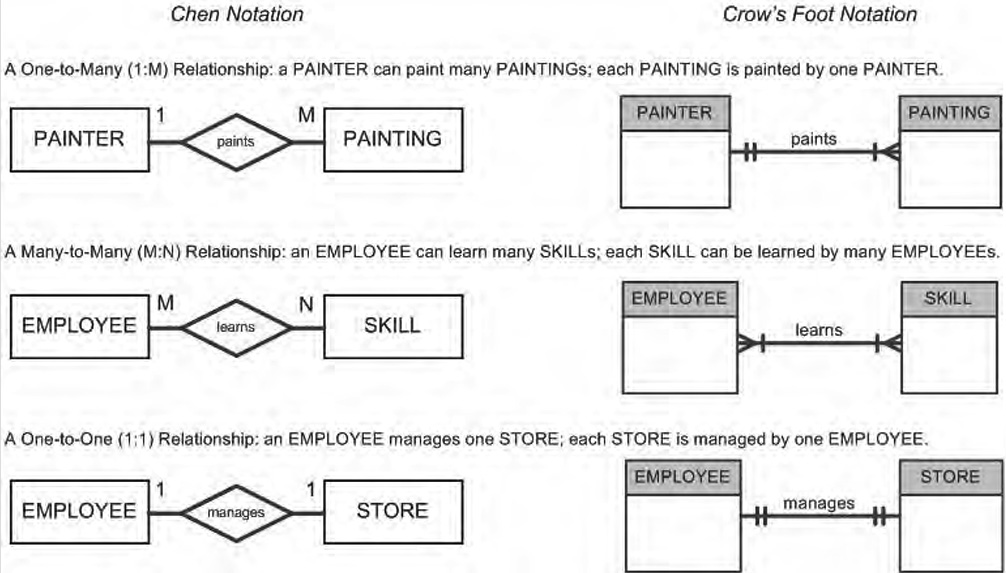
\includegraphics[width=1\linewidth]{../assets/chen-crowsfoot-notation.jpg}

\end{enumerate}
